\part{Travaux subséquents}

\chapter{Extension des fonctionnalités offertes}

    \section{Amélioration de la performance du modèle}

    Même si les résultats se montrent désormais très encourageants, il reste encore quelques améliorations à apporter pour que les utilisateurs y trouvent un réel intérêt.
    Avec une accuracy à 27\%, il y a encore trop de corrections manuelles à apporter.
    Pour chacune des pistes d'amélioration identifiées, il faudra évidemment procéder à une vérification de l'impact via une cross validation sur le set d'entraînement.

    \subsection{Découpage du contenu des documents en blocs de textes}

    L'essentiel des erreurs vient de soucis sur le découpage du texte en blocs.
    Cela dégrade à la fois la performance en termes de similarité et d'accuracy, mais pénalise également a fonctionnalité d'identification du meilleur candidat.
    Plusieurs pistes d'amélioration sont offertes pour améliorer ce point : 
    \begin{itemize}
        \item analyser les cas d'erreurs, et complexifier un peu l'expression régulière servant à découper le texte des documents en blocs
        \item multiplier les candidats pour une même fiche technique : on pourrait appliquer plusieurs fonctions de découpage différentes sur le document, et proposer l'ensemble des candidats obtenus au sélecteur
        \item dans la même logique, la constitution de \og ngrams de blocs \fg pourrait compenser les cas de mauvais découpages car trop fins, et multiplierait également le nombre de candidats proposés au sélecteur
        \item enfin, il faudrait se pencher sur les fonctionnalités de clustering des objets (caractères en mots, mots en lignes, lignes en paragraphes) proposées par les bibliothèques de mining de pdf. Les blocs candidats pourraient correspondre aux paragraphes identifiés par l'outil de mining.
    \end{itemize}

    De plus, il apparaît qu'une partie des écarts se situent en début ou en fin de texte (préfixes conservés alors qu'il aurait fallu les supprimer, mentions connexes non supprimées, \dots)
    pourrait être corrigés s'il était possible de \og tailler \fg le début et la fin du texte.
    On pourrait là encore procéder par apprentissage en déterminant : 
    \begin{itemize}
        \item une liste de mentions qui améliorent la performance lorsqu'elles sont retirées
        \item d'autres critères (document frequency dans les textes des fiches techniques, document frequency dans les listes d'ingrédients, \dots)
    \end{itemize}

    \subsection{Amélioration de l'identification par similarité}

    Dans les résultats sur le set de test, il reste encore des blocs incorrectement identifiés alors que la liste d'ingrédients était bien présente par ailleurs.
    Même si l'écart entre similarité cosinus et projection est important, on suspecte qu'il existe des manières plus performantes d'ajuster la manière de représenter les textes.
    En particulier, l'utilisation du scoring relatif (cf. section \mref{word_scores}) semblait prometteuse.
    Peut-être que tester une version où les scores relatifs sont calculés pour ne pas décaler les produits scalaires des candidats vers les valeurs négatives en moyenne pourrait être pertinente.

    Une autre piste serait de faire tourner en parallèles plusieurs sélecteurs de blocs, et d'appliquer une méthode ensembliste en les faisant voter pour le meilleur candidat.
    La performance du modèle est bonne sur les produits dont les listes d'ingrédients sont relativement longues, mais moins pertinente pour les produits plus bruts.
    L'identification d'un modèle performant sur les listes d'ingrédients courtes permettrait de pallier ce point et il faudrait l'associer au modèle actuel.

    \subsection{Filtrage des similarités trop basses}
    
    Un irritant majeur pour les utilisateurs est d'avoir un résultat complètement impertinent.
    Il serait intéressant d'identifier les cas où le modèle a retourné un candidat qui ne correspond pas à une liste d'ingrédients.
    On pourrait ensuite filtrer la proposition, et afficher à l'utilisateur que le traitement a échoué et que le modèle n'a pas réussi à extraire la liste d'ingrédients du document soumis.
    Une telle fonctionnalité pourrait également améliorer la performance du modèle, en couvrant les cas où le document fourni ne comporte pas de liste d'ingrédients.
    Cela pourrait se faire :
    \begin{itemize}
        \item en fixant un seuil minimum de similarité (cosinus et/ou projection) 
        \item en utilisant d'autres critères (longueur du candidat, document frequency moyenne des mots qui le composent, \dots)
    \end{itemize}

    \section{Extension du périmètre couvert avec la méthode \og textuelle \fg}
    Avant de pouvoir mettre en production des fonctionnalités de types extraction de connaissance depuis des documents, il serait intéressant d'en étoffer le périmètre.
    L'approche présentée dans ce document consiste à interpréter uniquement le texte brut, sans avoir recours à des fonctionnalités de spatialisation au sein du document.

    \subsection{Prise en compte de nouveaux types de pièces jointes}
    Les étiquettes produit doivent porter l'ensemble des informations réglementaires (données nutritionnelles, composition, allergènes, \dots, cf. section \mref{etiquettes_produit}).
    Même si les étiquettes ont plus tendance à être des documents pdf dont le contenu textuel n'est pas extractible sans faire appel à des fonctionnalités d'OCR (cf. \reftable{tbl:empty_attached_files}), un potentiel accessible existe déjà.
    La performance de l'identification des listes d'ingrédients devrait être d'ailleurs assez bonne sur les étiquettes, dans la mesure où il s'agit de documents bien moins verbeux.

    \subsection{Utilisation d'outil d'OCR pour les pdf non structurés}
    L'utilisation d'outils d'OCR pourrait venir compléter les fonctionnalités de pdfminer.six, en permettant l'extraction des textes depuis les documents non structurés.
    La suite du traitement pourrait rester parfaitement identique, en traitant uniquement le contenu textuel extrait, sans notion de spatialisation.
    De plus, cela complémenterait parfaitement l'extension des fonctionnalités aux étiquettes produits.

    \subsection{\'{E}valuation de la performances sur d'autres familles de produits}
    Le modèle a été construit sur la base des données de la branche \'{E}piSaveurs (cf. la description des branches du groupe, en annexe \mref{les_branches}).
    Cette branche ne commercialise que des produits stockés à température ambiante (pas de produit frais ou surgelés).
    Il serait intéressant de tester ce modèle sur les données des autres branches du groupe, dans l'optique de vérifier que les fonctionnalités pourraient leur être étendues.
    Un point à vérifier sur cette extension serait si la performance serait meilleure en construisant des modèles séparés, en fonction de la famille de produit, ou un modèle général qui tournerait sur l'ensemble des données.

    Les produits de chimie (cf. annexe \mref{produits_nonal}), commercialisés par la branche \'{E}piSaveurs, font également l'objet d'une déclaration de composition obligatoire sur l'emballage.
    On pourrait envisager de faire la même évaluation du modèle sur ces produits.
    Comme les \og ingrédients \fg des produits de chimie sont différents de ceux des produits alimentaires, il faudrait faire un entraînement particulier sur leurs données.

    \subsection{Récupération des dénominations réglementaires}

    Il est un autre texte qui est normalement présent sur l'emballage et la fiche technique du produit : la dénomination réglementaire (cf. annexe \mref{libelles}).
    Il est envisageable de constuire un modèle qui aurait en charge de récupérer cette information depuis les fiches techniques, ou les étiquettes produit.
    Comme ces désignations sont en général plus courtes que les liste d'ingrédients, il faudrait prévoir d'ajuster les paramètres du modèle, avec une méthode similaire à ce qui a été fait et présenté au chapitre \mref{model_tuning} \og Ajustement des paramètres \fg.

    \section{Changement de méthode}

    Dans le cadre d'un use case en lien avec l'extraction de connaissance sur les produits depuis des documents pdf, on pourrait également envisager d'autres méthodes.
    Cela rendrait accessible un grand nombre d'autres fonctionnalités, voire d'autres cas d'usage, en lien ou non avec la gestion de l'information produit.

    \subsection{Mise en place d'outil de spatialisation des textes}
    
    C'est clairement le sujet le plus prometteur à tester, mais également un des plus complexes à mettre en \oe uvre.
    L'idée derrière la spatialisation est de réussir à associer les informations présentes dans les documents entre elles, en fonction de leurs position dans le document.
    Il s'agit clairement d'un tout nouveau sujet, on passerait d'une problématique de traitement du langage à du traitement d'image.
    Le sujet est vaste, et il faudrait être en mesure : 
    \begin{itemize}
        \item de détecter les tableaux présents dans les documents (voir par exemple la fiche technique des poivrons en annexe \mref{ex:FT_poivron}) : 
        \begin{itemize}
            \item puis de détecter les entêtes de lignes ou de colonnes, pour avoir une représentation à simple ou double entrée de l'information
            \item de construire les relations entre les niveaux hiéarchiques d'indexation dans ces tableaux (ex : Valeurs nutritionnelles > \'{E}nergie = 109 kJ)
        \end{itemize}
        \item de comprendre la structure du document, et les liens entre les titres entre les contenus des différentes sections (cf. la fiche technique de la panna cotta, en annexe \mref{ex:FT_pannacotta})
    \end{itemize}
    Il s'agit d'un sujet ambitieux, mais qui aurait en plus l'avantage de pouvoir être étendu à la quasi totalité des cas métier où des documents sont interprétés.
    Dans le cas précis de la gestion de l'information produit, cela permettrait d'aller récupérer les données nutritionnelles par exemple (cf. annexe \mref{donnees_nut}).

    \subsection{Aides pour le contrôle de cohérence}
    
    Toujours dans l'optique d'améliorer la qualité des données des produits, on pourrait changer de sujet et passer à des contrôles de cohérence entre les données elles-mêmes.
    Par exemple, il est normalement possible pour un utilisateur correctement formé de déterminer l'ensemble des allergènes du produit à la lecture de la liste d'ingrédients (sous réserve qu'elle mentionne bien également les contaminations croisées).
    On pourrait envisager de déterminer quels mots ou expressions parmi les listes d'ingrédients permettent d'identifier tel ou tel allergène réglementaire (cf. annexe \mref{composition} pour plus de détail sur les allergènes).

    Il serait également possible de déterminer, par des méthodes de classification, si un produit se qualifie pour une allégation nutritionnelle quelconque (ex : faible en sel), sur la base de ses données nutritionnelles, afin de contrôler si une allégation qui a été transmise par le fournisseur est cohérente.

    \chapter{Déploiement opérationnel de l'outil}    

        \section{Mise en place d'une organisation projet}
            
            \subsection{Sponsor et Client}

            La toute première étape pour le lancement d'un projet visant à mettre en \oe uvre ce modèle, serait d'indentifier un sponsor capable de mobiliser une enveloppe budgétaire, et de prendre les décisions de niveau stratégique.
            Ensuite, il faudrait identifier quelques représentants métier (gestionnaires de référentiel, ingénieurs qualité, acheteurs, \dots) qui seraient capable de se prononcer sur les règles de gestion et les décisions organisationnelles.
            Il est indispensable d'avoir ces deux niveaux engagés dans le projet dès son lancement.

            La toute première décision attendu du sponsor serait le choix du cas d'usage, tel que décrit au chapitre \mref{use_cases} sur le cas d'usage.
            Souhaite-t-on mettre à disposition des fonctionnalité de préalimentation des informations produit ou bien faciliter et fiabiliser le contrôle ?

            \subsection{Choix techniques et technologiques}

            Les autres grandes décisions à prendre en compte en début de projet sont d'ordre techniques et technologiques.
            La première est de savoir dans quel langage le modèle de production serait développé.
            Poursuivre en python aurait l'avantage de pouvoir capitaliser sur les travaux déjà effectués, et de se baser sur les bibliothèques qui ont fait leurs preuves (essentiellement numpy et scikit-learn).
            De plus, il faudrait dès le début du projet définir la criticité de ces fonctionnalités, et prévoir dès le départ le mode de redondance et l'éventuel plan de reprise d'activité.
            Enfin, même si les travaux effectués ont montré que le modèle en l'état était peu gourmand en mémoire et puissance de calcul, il faudrait extrapoler le dimensionnement nécessaire pour tenir la charge pour l'ensemble des branches du groupe.

            \subsection{Développement microservice}

            Tant la préalimentation, que l'aide au contrôle des données seraient implémentables comme un service.
            Il suffirait pour cela de publier un service, qui fonctionnerait de la manière suivante (illustré à la \reffig{fig:sequence_diag}) : 
            \begin{itemize}
                \item le PIM appelle le service, avec un message contenant l'uid du produit à contrôler ou préalimenter
                \item le serveur récupère du PIM les données nécessaires au contrôle ou à la préalimentation
                \item en retour, il renvoie au PIM soit l'état du contrôle (OK, erreur, avertissement, avec les précisions nécessaires), soit les données telles qu'elles doivent être préalimentées
                \item le PIM, sur la base de ce retour, affiche le résultat du contrôle ou bien alimente les données et les présente à l'utilisateur
            \end{itemize}

            \begin{figure}[htbp]
                \begin{center}
                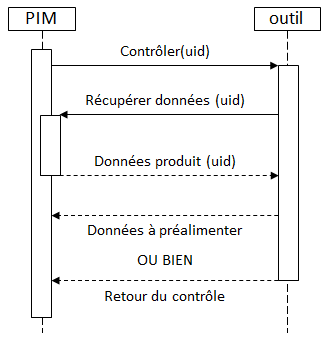
\includegraphics[width=0.4\linewidth]{img/sequence_diag.png}
                \end{center}
                \caption{Diagramme de séquence des échanges entre PIM et le service}
                \label{fig:sequence_diag}
            \end{figure}

            Ce mode de fonctionnement nécessiterait des développements supplémentaires au niveau du PIM : 
            \begin{itemize}
                \item appel du service lorsque les conditions sont réunies (ex : lancement du contrôle des données par l'acheteur)
                \item intégration des données retournées si le cas d'usage est la préalimentation
                \item affichage à l'utilisateur du résultat du contrôle si le cas d'usage est l'appui au contrôle
            \end{itemize}

        \section{Maintien en condition opérationnelle}

            \subsection{Mise à niveau}
            
            Si le projet devait se poursuivre en python, afin de disposer d'un outil restant maintenu au fil du temps, il est nécessaire d'industrialiser ce prototype.
            Pour cela, il faudrait : 
            \begin{itemize}
                \item procéder au refactoring de certaines classes. Le requester porte trop de responsabilités (requêtage des données du PIM, conversion en DataFrame, conservation persistantes des données stockées localement, \dots) et devrait être séparé en classes plus petites. Le calcul de similarité par projection devrait être réécrit, pour éviter d'utiliser deux TFIDFVectorizer, mais plutôt d'effectuer une projection par produit de matrices.
                \item mettre en place les fonctionnalités de typage statique
                \item poursuivre la rédaction de tests unitaires, avec une cible de couverture à 80\%
                \item revoir ou réécrire l'ensemble des docstrings, et générer la documentation du code via des outils tels que Sphinx
            \end{itemize}

            \subsection{Intégration et déploiement continu}

            En parallèle de l'écriture des tests et du passage au typage statique, il faudrait mettre en place un pipeline d'intégration et déploiement continu.
            Celui-ci permettrait d'identifier au plus tôt les problèmes en :
            \begin{itemize}
                \item procédant dès la production du code à la vérification du typage
                \item contrôlant la qualité de l'écriture du code (linting)
                \item faisant tourner les tests unitaires pour éviter les régressions
            \end{itemize}
            Le déploiement continu permettrait de mettre à disposition régulièrement et rapidement les améliorations et corrections aux utilisateurs

            \subsection{Monitoring de la performance du modèle}

            Un point crucial pour que le projet soit un succès est la surveillance de la performance du modèle.
            Il est possible que des dérives apparaissent, par exemple si au fil du temps les caractéristiques des données étaient modifiées (par exemple, de nouvelles manières de nommer les ingréidents apparaissaient, les règles de gestion changeaient, \dots).
            Il faudrait être capable d'identifier ce phénomène, pour pouvoir prendre les actions correctrices nécessaires : 
            \begin{itemize}
                \item changement des paramètres du modèle
                \item réentrainement sur des données plus récentes
                \item construction de nouveaux modèles pour gérer des domaines spécifiques
            \end{itemize}
            Un point à trancher est la manière de monitorer la performance.
            Une façon de faire serait de capturer les décisions prises par les utilisateurs après que le modèle a tourné.
            Par exemple, dans le cadre de l'aide au contrôle, est-ce que l'utilisateur a décidé de passer outre l'avertissement qui lui a été remonté par le système ?
            Dans le cas de la préalimentation d'information, l'utilisateur a-t-il corrigé la valeur qui lui a été fournie ?
            Ces décisions devraient être enregistrées, puis analysées afin de s'assurer que la performance du modèle ne se dégrade pas au fil du temps.
            
            \section{Conclusion}

            Les résultats obtenus démontrent la faisabilité de la mise en place d'un outil d'extraction automatique de connaissance depuis des documents.
            Même s'il reste encore des travaux à mener avant de pouvoir déployer un outil apportant de la valeur au groupe, ce démonstrateur permet d'illustrer les fonctionnalités rendues accessibles par l'analyse de données et le machine learning.
            Cette ouverture, si elle est partagée avec le management du Groupe Pomona, peut permettre le lancement de nombreux projets innovants et porteurs de valeur.